\documentclass{standalone}
\usepackage{tikz}
\usetikzlibrary{patterns, positioning}

\begin{document}
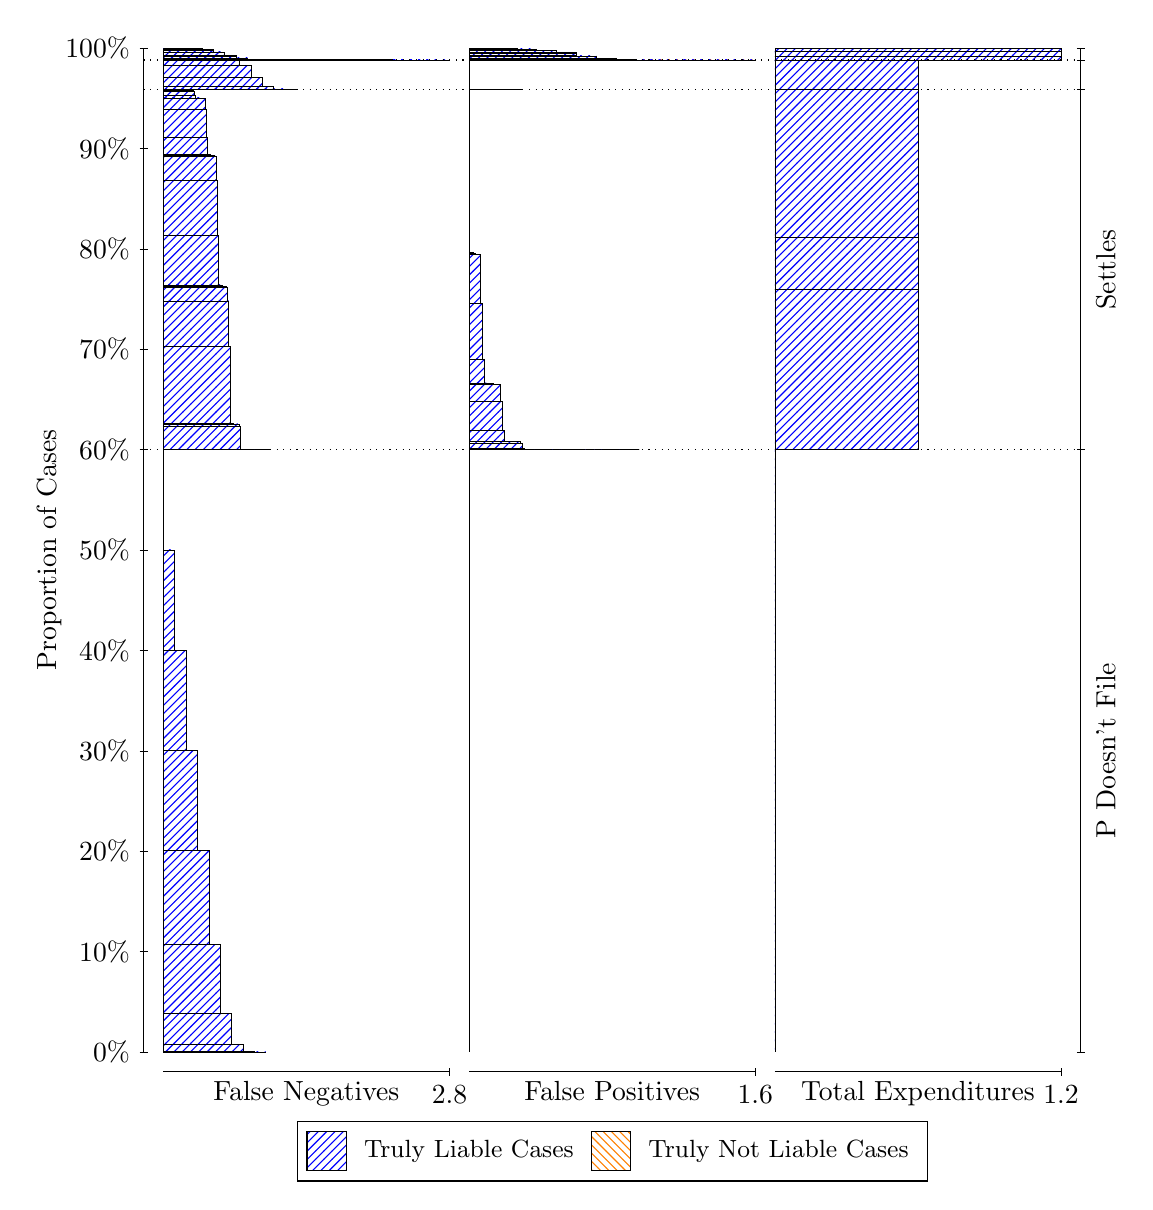
\begin{tikzpicture}
\draw[black, very thin] (1.5,1.75) -- (1.5,14.5);
\node[rotate=90, anchor=center] at (0.3, 8.125) {Proportion of Cases};
\draw[black, very thin] (1.45,1.75) -- (1.55,1.75);
\node[anchor=east] at (1.45, 1.75) {0\%};
\draw[black, very thin] (1.45,3.025) -- (1.55,3.025);
\node[anchor=east] at (1.45, 3.025) {10\%};
\draw[black, very thin] (1.45,4.3) -- (1.55,4.3);
\node[anchor=east] at (1.45, 4.3) {20\%};
\draw[black, very thin] (1.45,5.575) -- (1.55,5.575);
\node[anchor=east] at (1.45, 5.575) {30\%};
\draw[black, very thin] (1.45,6.85) -- (1.55,6.85);
\node[anchor=east] at (1.45, 6.85) {40\%};
\draw[black, very thin] (1.45,8.125) -- (1.55,8.125);
\node[anchor=east] at (1.45, 8.125) {50\%};
\draw[black, very thin] (1.45,9.4) -- (1.55,9.4);
\node[anchor=east] at (1.45, 9.4) {60\%};
\draw[black, very thin] (1.45,10.675) -- (1.55,10.675);
\node[anchor=east] at (1.45, 10.675) {70\%};
\draw[black, very thin] (1.45,11.95) -- (1.55,11.95);
\node[anchor=east] at (1.45, 11.95) {80\%};
\draw[black, very thin] (1.45,13.225) -- (1.55,13.225);
\node[anchor=east] at (1.45, 13.225) {90\%};
\draw[black, very thin] (1.45,14.5) -- (1.55,14.5);
\node[anchor=east] at (1.45, 14.5) {100\%};

\draw[black, very thin] (13.4,1.75) -- (13.4,14.5);
\draw[black, very thin] (13.35,1.75) -- (13.45,1.75);
\node[anchor=west] at (13.35, 1.75) {};
\draw[black, very thin] (13.35,9.4013) -- (13.45,9.4013);
\node[anchor=west] at (13.35, 9.4013) {};
\draw[black, very thin] (13.35,13.971) -- (13.45,13.971);
\node[anchor=west] at (13.35, 13.971) {};
\draw[black, very thin] (13.35,14.347) -- (13.45,14.347);
\node[anchor=west] at (13.35, 14.347) {};
\draw[black, very thin] (13.35,14.349) -- (13.45,14.349);
\node[anchor=west] at (13.35, 14.349) {};
\draw[black, very thin] (13.35,14.5) -- (13.45,14.5);
\node[anchor=west] at (13.35, 14.5) {};

\draw[black, very thin, pattern color=blue, pattern=north east lines] (1.75,1.75) rectangle (3.0476,1.7504);
\draw[black, very thin, pattern color=blue, pattern=north east lines] (1.75,1.7504) rectangle (2.9034,1.7589);
\draw[black, very thin, pattern color=blue, pattern=north east lines] (1.75,1.7589) rectangle (2.7593,1.8446);
\draw[black, very thin, pattern color=blue, pattern=north east lines] (1.75,1.8446) rectangle (2.6151,2.2381);
\draw[black, very thin, pattern color=blue, pattern=north east lines] (1.75,2.2381) rectangle (2.4709,3.1197);
\draw[black, very thin, pattern color=blue, pattern=north east lines] (1.75,3.1197) rectangle (2.3267,4.3095);
\draw[black, very thin, pattern color=blue, pattern=north east lines] (1.75,4.3095) rectangle (2.1825,5.5766);
\draw[black, very thin, pattern color=blue, pattern=north east lines] (1.75,5.5766) rectangle (2.0384,6.8513);
\draw[black, very thin, pattern color=blue, pattern=north east lines] (1.75,6.8513) rectangle (1.8942,8.1263);
\draw[black, very thin, pattern color=orange, pattern=north west lines] (1.75,8.1263) rectangle (1.75,8.1263);
\draw[black, very thin, pattern color=blue, pattern=north east lines] (1.75,8.1263) rectangle (1.75,9.4013);
\draw[black, very thin, pattern color=blue, pattern=north east lines] (1.75,9.4013) rectangle (3.1125,9.4013);
\draw[black, very thin, pattern color=blue, pattern=north east lines] (1.75,9.4013) rectangle (3.0476,9.4013);
\draw[black, very thin, pattern color=blue, pattern=north east lines] (1.75,9.4013) rectangle (2.9827,9.4013);
\draw[black, very thin, pattern color=blue, pattern=north east lines] (1.75,9.4013) rectangle (2.9683,9.4013);
\draw[black, very thin, pattern color=blue, pattern=north east lines] (1.75,9.4013) rectangle (2.9179,9.4013);
\draw[black, very thin, pattern color=blue, pattern=north east lines] (1.75,9.4013) rectangle (2.9034,9.4013);
\draw[black, very thin, pattern color=blue, pattern=north east lines] (1.75,9.4013) rectangle (2.853,9.4032);
\draw[black, very thin, pattern color=blue, pattern=north east lines] (1.75,9.4032) rectangle (2.8386,9.4033);
\draw[black, very thin, pattern color=blue, pattern=north east lines] (1.75,9.4033) rectangle (2.8241,9.4034);
\draw[black, very thin, pattern color=blue, pattern=north east lines] (1.75,9.4034) rectangle (2.7881,9.4039);
\draw[black, very thin, pattern color=blue, pattern=north east lines] (1.75,9.4039) rectangle (2.7737,9.4041);
\draw[black, very thin, pattern color=blue, pattern=north east lines] (1.75,9.4041) rectangle (2.7593,9.4043);
\draw[black, very thin, pattern color=blue, pattern=north east lines] (1.75,9.4043) rectangle (2.7232,9.6948);
\draw[black, very thin, pattern color=blue, pattern=north east lines] (1.75,9.6948) rectangle (2.7088,9.7234);
\draw[black, very thin, pattern color=blue, pattern=north east lines] (1.75,9.7234) rectangle (2.6944,9.7255);
\draw[black, very thin, pattern color=blue, pattern=north east lines] (1.75,9.7255) rectangle (2.68,9.7262);
\draw[black, very thin, pattern color=blue, pattern=north east lines] (1.75,9.7262) rectangle (2.6439,9.7301);
\draw[black, very thin, pattern color=blue, pattern=north east lines] (1.75,9.7301) rectangle (2.6295,9.7329);
\draw[black, very thin, pattern color=blue, pattern=north east lines] (1.75,9.7329) rectangle (2.6151,9.734);
\draw[black, very thin, pattern color=blue, pattern=north east lines] (1.75,9.734) rectangle (2.5935,10.71);
\draw[black, very thin, pattern color=blue, pattern=north east lines] (1.75,10.71) rectangle (2.579,11.289);
\draw[black, very thin, pattern color=blue, pattern=north east lines] (1.75,11.289) rectangle (2.5646,11.461);
\draw[black, very thin, pattern color=blue, pattern=north east lines] (1.75,11.461) rectangle (2.5502,11.468);
\draw[black, very thin, pattern color=blue, pattern=north east lines] (1.75,11.468) rectangle (2.5358,11.47);
\draw[black, very thin, pattern color=blue, pattern=north east lines] (1.75,11.47) rectangle (2.4997,11.482);
\draw[black, very thin, pattern color=blue, pattern=north east lines] (1.75,11.482) rectangle (2.4853,11.492);
\draw[black, very thin, pattern color=blue, pattern=north east lines] (1.75,11.492) rectangle (2.4709,11.493);
\draw[black, very thin, pattern color=blue, pattern=north east lines] (1.75,11.493) rectangle (2.4493,12.117);
\draw[black, very thin, pattern color=blue, pattern=north east lines] (1.75,12.117) rectangle (2.4349,12.82);
\draw[black, very thin, pattern color=blue, pattern=north east lines] (1.75,12.82) rectangle (2.4204,13.125);
\draw[black, very thin, pattern color=blue, pattern=north east lines] (1.75,13.125) rectangle (2.406,13.131);
\draw[black, very thin, pattern color=blue, pattern=north east lines] (1.75,13.131) rectangle (2.3916,13.132);
\draw[black, very thin, pattern color=blue, pattern=north east lines] (1.75,13.132) rectangle (2.3556,13.143);
\draw[black, very thin, pattern color=blue, pattern=north east lines] (1.75,13.143) rectangle (2.3411,13.149);
\draw[black, very thin, pattern color=blue, pattern=north east lines] (1.75,13.149) rectangle (2.3267,13.149);
\draw[black, very thin, pattern color=blue, pattern=north east lines] (1.75,13.149) rectangle (2.3051,13.361);
\draw[black, very thin, pattern color=blue, pattern=north east lines] (1.75,13.361) rectangle (2.2907,13.724);
\draw[black, very thin, pattern color=blue, pattern=north east lines] (1.75,13.724) rectangle (2.2763,13.864);
\draw[black, very thin, pattern color=blue, pattern=north east lines] (1.75,13.864) rectangle (2.2618,13.865);
\draw[black, very thin, pattern color=blue, pattern=north east lines] (1.75,13.865) rectangle (2.2474,13.865);
\draw[black, very thin, pattern color=blue, pattern=north east lines] (1.75,13.865) rectangle (2.2114,13.867);
\draw[black, very thin, pattern color=blue, pattern=north east lines] (1.75,13.867) rectangle (2.197,13.868);
\draw[black, very thin, pattern color=blue, pattern=north east lines] (1.75,13.868) rectangle (2.1825,13.868);
\draw[black, very thin, pattern color=blue, pattern=north east lines] (1.75,13.868) rectangle (2.1609,13.894);
\draw[black, very thin, pattern color=blue, pattern=north east lines] (1.75,13.894) rectangle (2.1465,13.953);
\draw[black, very thin, pattern color=blue, pattern=north east lines] (1.75,13.953) rectangle (2.1321,13.968);
\draw[black, very thin, pattern color=blue, pattern=north east lines] (1.75,13.968) rectangle (2.1177,13.968);
\draw[black, very thin, pattern color=blue, pattern=north east lines] (1.75,13.968) rectangle (2.1032,13.968);
\draw[black, very thin, pattern color=blue, pattern=north east lines] (1.75,13.968) rectangle (2.0672,13.968);
\draw[black, very thin, pattern color=blue, pattern=north east lines] (1.75,13.968) rectangle (2.0528,13.968);
\draw[black, very thin, pattern color=blue, pattern=north east lines] (1.75,13.968) rectangle (2.0384,13.968);
\draw[black, very thin, pattern color=blue, pattern=north east lines] (1.75,13.968) rectangle (2.0167,13.969);
\draw[black, very thin, pattern color=blue, pattern=north east lines] (1.75,13.969) rectangle (2.0023,13.971);
\draw[black, very thin, pattern color=blue, pattern=north east lines] (1.75,13.971) rectangle (1.9879,13.971);
\draw[black, very thin, pattern color=blue, pattern=north east lines] (1.75,13.971) rectangle (1.9735,13.971);
\draw[black, very thin, pattern color=blue, pattern=north east lines] (1.75,13.971) rectangle (1.9591,13.971);
\draw[black, very thin, pattern color=blue, pattern=north east lines] (1.75,13.971) rectangle (1.923,13.971);
\draw[black, very thin, pattern color=blue, pattern=north east lines] (1.75,13.971) rectangle (1.9086,13.971);
\draw[black, very thin, pattern color=blue, pattern=north east lines] (1.75,13.971) rectangle (1.8942,13.971);
\draw[black, very thin, pattern color=blue, pattern=north east lines] (1.75,13.971) rectangle (1.8726,13.971);
\draw[black, very thin, pattern color=blue, pattern=north east lines] (1.75,13.971) rectangle (1.8581,13.971);
\draw[black, very thin, pattern color=blue, pattern=north east lines] (1.75,13.971) rectangle (1.8437,13.971);
\draw[black, very thin, pattern color=blue, pattern=north east lines] (1.75,13.971) rectangle (1.8293,13.971);
\draw[black, very thin, pattern color=blue, pattern=north east lines] (1.75,13.971) rectangle (1.8149,13.971);
\draw[black, very thin, pattern color=blue, pattern=north east lines] (1.75,13.971) rectangle (1.7788,13.971);
\draw[black, very thin, pattern color=blue, pattern=north east lines] (1.75,13.971) rectangle (1.7644,13.971);
\draw[black, very thin, pattern color=orange, pattern=north west lines] (1.75,13.971) rectangle (1.75,13.971);
\draw[black, very thin, pattern color=blue, pattern=north east lines] (1.75,13.971) rectangle (1.75,13.971);
\draw[black, very thin, pattern color=blue, pattern=north east lines] (1.75,13.971) rectangle (3.4369,13.972);
\draw[black, very thin, pattern color=blue, pattern=north east lines] (1.75,13.972) rectangle (3.2927,13.98);
\draw[black, very thin, pattern color=blue, pattern=north east lines] (1.75,13.98) rectangle (3.1485,14.016);
\draw[black, very thin, pattern color=blue, pattern=north east lines] (1.75,14.016) rectangle (3.0044,14.125);
\draw[black, very thin, pattern color=blue, pattern=north east lines] (1.75,14.125) rectangle (2.8602,14.278);
\draw[black, very thin, pattern color=blue, pattern=north east lines] (1.75,14.278) rectangle (2.716,14.339);
\draw[black, very thin, pattern color=blue, pattern=north east lines] (1.75,14.339) rectangle (2.5718,14.347);
\draw[black, very thin, pattern color=blue, pattern=north east lines] (1.75,14.347) rectangle (2.4276,14.347);
\draw[black, very thin, pattern color=blue, pattern=north east lines] (1.75,14.347) rectangle (2.2835,14.347);
\draw[black, very thin, pattern color=blue, pattern=north east lines] (1.75,14.347) rectangle (2.1393,14.347);
\draw[black, very thin, pattern color=orange, pattern=north west lines] (1.75,14.347) rectangle (1.75,14.347);
\draw[black, very thin, pattern color=blue, pattern=north east lines] (1.75,14.347) rectangle (2.1393,14.347);
\draw[black, very thin, pattern color=blue, pattern=north east lines] (1.75,14.347) rectangle (1.9951,14.348);
\draw[black, very thin, pattern color=blue, pattern=north east lines] (1.75,14.348) rectangle (1.8509,14.349);
\draw[black, very thin, pattern color=orange, pattern=north west lines] (1.75,14.349) rectangle (1.75,14.349);
\draw[black, very thin, pattern color=blue, pattern=north east lines] (1.75,14.349) rectangle (1.75,14.349);
\draw[black, very thin, pattern color=blue, pattern=north east lines] (1.75,14.349) rectangle (5.3833,14.349);
\draw[black, very thin, pattern color=blue, pattern=north east lines] (1.75,14.349) rectangle (5.2392,14.349);
\draw[black, very thin, pattern color=blue, pattern=north east lines] (1.75,14.349) rectangle (5.095,14.349);
\draw[black, very thin, pattern color=blue, pattern=north east lines] (1.75,14.349) rectangle (4.9508,14.349);
\draw[black, very thin, pattern color=blue, pattern=north east lines] (1.75,14.349) rectangle (4.9508,14.349);
\draw[black, very thin, pattern color=blue, pattern=north east lines] (1.75,14.349) rectangle (4.8066,14.349);
\draw[black, very thin, pattern color=blue, pattern=north east lines] (1.75,14.349) rectangle (4.6624,14.35);
\draw[black, very thin, pattern color=blue, pattern=north east lines] (1.75,14.35) rectangle (4.6624,14.351);
\draw[black, very thin, pattern color=blue, pattern=north east lines] (1.75,14.351) rectangle (4.5183,14.353);
\draw[black, very thin, pattern color=blue, pattern=north east lines] (1.75,14.353) rectangle (4.5183,14.354);
\draw[black, very thin, pattern color=blue, pattern=north east lines] (1.75,14.354) rectangle (4.3741,14.356);
\draw[black, very thin, pattern color=blue, pattern=north east lines] (1.75,14.356) rectangle (4.2299,14.356);
\draw[black, very thin, pattern color=blue, pattern=north east lines] (1.75,14.356) rectangle (4.2299,14.356);
\draw[black, very thin, pattern color=blue, pattern=north east lines] (1.75,14.356) rectangle (4.0857,14.356);
\draw[black, very thin, pattern color=blue, pattern=north east lines] (1.75,14.356) rectangle (3.9415,14.356);
\draw[black, very thin, pattern color=blue, pattern=north east lines] (1.75,14.356) rectangle (3.7974,14.356);
\draw[black, very thin, pattern color=blue, pattern=north east lines] (1.75,14.356) rectangle (3.7974,14.356);
\draw[black, very thin, pattern color=blue, pattern=north east lines] (1.75,14.356) rectangle (3.6532,14.356);
\draw[black, very thin, pattern color=blue, pattern=north east lines] (1.75,14.356) rectangle (3.5378,14.356);
\draw[black, very thin, pattern color=blue, pattern=north east lines] (1.75,14.356) rectangle (3.509,14.356);
\draw[black, very thin, pattern color=blue, pattern=north east lines] (1.75,14.356) rectangle (3.3937,14.356);
\draw[black, very thin, pattern color=blue, pattern=north east lines] (1.75,14.356) rectangle (3.2495,14.356);
\draw[black, very thin, pattern color=blue, pattern=north east lines] (1.75,14.356) rectangle (3.1053,14.356);
\draw[black, very thin, pattern color=blue, pattern=north east lines] (1.75,14.356) rectangle (3.1053,14.356);
\draw[black, very thin, pattern color=blue, pattern=north east lines] (1.75,14.356) rectangle (2.9611,14.358);
\draw[black, very thin, pattern color=blue, pattern=north east lines] (1.75,14.358) rectangle (2.9611,14.359);
\draw[black, very thin, pattern color=blue, pattern=north east lines] (1.75,14.359) rectangle (2.8169,14.375);
\draw[black, very thin, pattern color=blue, pattern=north east lines] (1.75,14.375) rectangle (2.6728,14.392);
\draw[black, very thin, pattern color=blue, pattern=north east lines] (1.75,14.392) rectangle (2.6728,14.409);
\draw[black, very thin, pattern color=blue, pattern=north east lines] (1.75,14.409) rectangle (2.5286,14.45);
\draw[black, very thin, pattern color=blue, pattern=north east lines] (1.75,14.45) rectangle (2.3844,14.466);
\draw[black, very thin, pattern color=blue, pattern=north east lines] (1.75,14.466) rectangle (2.3844,14.466);
\draw[black, very thin, pattern color=blue, pattern=north east lines] (1.75,14.466) rectangle (2.3844,14.483);
\draw[black, very thin, pattern color=blue, pattern=north east lines] (1.75,14.483) rectangle (2.2402,14.497);
\draw[black, very thin, pattern color=blue, pattern=north east lines] (1.75,14.497) rectangle (2.2402,14.497);
\draw[black, very thin, pattern color=blue, pattern=north east lines] (1.75,14.497) rectangle (2.096,14.498);
\draw[black, very thin, pattern color=blue, pattern=north east lines] (1.75,14.498) rectangle (2.096,14.498);
\draw[black, very thin, pattern color=blue, pattern=north east lines] (1.75,14.498) rectangle (2.096,14.5);
\draw[black, very thin, pattern color=blue, pattern=north east lines] (1.75,14.5) rectangle (1.9519,14.5);
\draw[black, very thin, pattern color=blue, pattern=north east lines] (1.75,14.5) rectangle (1.9519,14.5);
\draw[black, very thin, pattern color=blue, pattern=north east lines] (1.75,14.5) rectangle (1.8077,14.5);
\draw[black, very thin, pattern color=blue, pattern=north east lines] (1.75,14.5) rectangle (1.8077,14.5);
\draw[black, very thin, pattern color=orange, pattern=north west lines] (1.75,14.5) rectangle (1.75,14.5);
\draw[black, very thin, pattern color=blue, pattern=north east lines] (1.75,14.5) rectangle (1.75,14.5);
\draw[black, very thin, pattern color=orange, pattern=north west lines] (5.6333,1.75) rectangle (5.6333,1.75);
\draw[black, very thin, pattern color=blue, pattern=north east lines] (5.6333,1.75) rectangle (5.6333,9.4013);
\draw[black, very thin, pattern color=orange, pattern=north west lines] (5.6333,9.4013) rectangle (7.7906,9.4013);
\draw[black, very thin, pattern color=blue, pattern=north east lines] (5.6333,9.4013) rectangle (7.7906,9.4013);
\draw[black, very thin, pattern color=orange, pattern=north west lines] (5.6333,9.4013) rectangle (7.5635,9.4013);
\draw[black, very thin, pattern color=blue, pattern=north east lines] (5.6333,9.4013) rectangle (7.5635,9.4013);
\draw[black, very thin, pattern color=blue, pattern=north east lines] (5.6333,9.4013) rectangle (7.5383,9.4013);
\draw[black, very thin, pattern color=orange, pattern=north west lines] (5.6333,9.4013) rectangle (7.45,9.4013);
\draw[black, very thin, pattern color=blue, pattern=north east lines] (5.6333,9.4013) rectangle (7.45,9.4013);
\draw[black, very thin, pattern color=orange, pattern=north west lines] (5.6333,9.4013) rectangle (7.3365,9.4013);
\draw[black, very thin, pattern color=blue, pattern=north east lines] (5.6333,9.4013) rectangle (7.3365,9.4013);
\draw[black, very thin, pattern color=blue, pattern=north east lines] (5.6333,9.4013) rectangle (7.3112,9.4013);
\draw[black, very thin, pattern color=blue, pattern=north east lines] (5.6333,9.4013) rectangle (7.286,9.4013);
\draw[black, very thin, pattern color=orange, pattern=north west lines] (5.6333,9.4013) rectangle (7.2229,9.4013);
\draw[black, very thin, pattern color=blue, pattern=north east lines] (5.6333,9.4013) rectangle (7.2229,9.4013);
\draw[black, very thin, pattern color=blue, pattern=north east lines] (5.6333,9.4013) rectangle (7.1977,9.4013);
\draw[black, very thin, pattern color=orange, pattern=north west lines] (5.6333,9.4013) rectangle (7.1094,9.4013);
\draw[black, very thin, pattern color=blue, pattern=north east lines] (5.6333,9.4013) rectangle (7.1094,9.4013);
\draw[black, very thin, pattern color=blue, pattern=north east lines] (5.6333,9.4013) rectangle (7.0841,9.4013);
\draw[black, very thin, pattern color=blue, pattern=north east lines] (5.6333,9.4013) rectangle (7.0589,9.4013);
\draw[black, very thin, pattern color=blue, pattern=north east lines] (5.6333,9.4013) rectangle (7.0337,9.4013);
\draw[black, very thin, pattern color=orange, pattern=north west lines] (5.6333,9.4013) rectangle (6.9958,9.4013);
\draw[black, very thin, pattern color=blue, pattern=north east lines] (5.6333,9.4013) rectangle (6.9958,9.4013);
\draw[black, very thin, pattern color=blue, pattern=north east lines] (5.6333,9.4013) rectangle (6.9706,9.4013);
\draw[black, very thin, pattern color=blue, pattern=north east lines] (5.6333,9.4013) rectangle (6.9454,9.4013);
\draw[black, very thin, pattern color=orange, pattern=north west lines] (5.6333,9.4013) rectangle (6.8823,9.4013);
\draw[black, very thin, pattern color=blue, pattern=north east lines] (5.6333,9.4013) rectangle (6.8823,9.4013);
\draw[black, very thin, pattern color=blue, pattern=north east lines] (5.6333,9.4013) rectangle (6.8571,9.4013);
\draw[black, very thin, pattern color=blue, pattern=north east lines] (5.6333,9.4013) rectangle (6.8318,9.4013);
\draw[black, very thin, pattern color=blue, pattern=north east lines] (5.6333,9.4013) rectangle (6.8066,9.4013);
\draw[black, very thin, pattern color=blue, pattern=north east lines] (5.6333,9.4013) rectangle (6.7814,9.4013);
\draw[black, very thin, pattern color=blue, pattern=north east lines] (5.6333,9.4013) rectangle (6.7435,9.4013);
\draw[black, very thin, pattern color=blue, pattern=north east lines] (5.6333,9.4013) rectangle (6.7183,9.4013);
\draw[black, very thin, pattern color=blue, pattern=north east lines] (5.6333,9.4013) rectangle (6.6931,9.4013);
\draw[black, very thin, pattern color=blue, pattern=north east lines] (5.6333,9.4013) rectangle (6.63,9.4013);
\draw[black, very thin, pattern color=blue, pattern=north east lines] (5.6333,9.4013) rectangle (6.6047,9.4013);
\draw[black, very thin, pattern color=blue, pattern=north east lines] (5.6333,9.4013) rectangle (6.5795,9.4016);
\draw[black, very thin, pattern color=blue, pattern=north east lines] (5.6333,9.4016) rectangle (6.5543,9.404);
\draw[black, very thin, pattern color=blue, pattern=north east lines] (5.6333,9.404) rectangle (6.5291,9.4048);
\draw[black, very thin, pattern color=blue, pattern=north east lines] (5.6333,9.4048) rectangle (6.4912,9.4048);
\draw[black, very thin, pattern color=blue, pattern=north east lines] (5.6333,9.4048) rectangle (6.466,9.4048);
\draw[black, very thin, pattern color=blue, pattern=north east lines] (5.6333,9.4048) rectangle (6.4407,9.405);
\draw[black, very thin, pattern color=blue, pattern=north east lines] (5.6333,9.405) rectangle (6.3777,9.405);
\draw[black, very thin, pattern color=blue, pattern=north east lines] (5.6333,9.405) rectangle (6.3524,9.405);
\draw[black, very thin, pattern color=blue, pattern=north east lines] (5.6333,9.405) rectangle (6.3272,9.4196);
\draw[black, very thin, pattern color=blue, pattern=north east lines] (5.6333,9.4196) rectangle (6.302,9.4791);
\draw[black, very thin, pattern color=blue, pattern=north east lines] (5.6333,9.4791) rectangle (6.2767,9.5047);
\draw[black, very thin, pattern color=blue, pattern=north east lines] (5.6333,9.5047) rectangle (6.2389,9.5047);
\draw[black, very thin, pattern color=blue, pattern=north east lines] (5.6333,9.5047) rectangle (6.2137,9.5054);
\draw[black, very thin, pattern color=blue, pattern=north east lines] (5.6333,9.5054) rectangle (6.1884,9.5079);
\draw[black, very thin, pattern color=blue, pattern=north east lines] (5.6333,9.5079) rectangle (6.1253,9.508);
\draw[black, very thin, pattern color=blue, pattern=north east lines] (5.6333,9.508) rectangle (6.1001,9.5087);
\draw[black, very thin, pattern color=blue, pattern=north east lines] (5.6333,9.5087) rectangle (6.0749,9.6486);
\draw[black, very thin, pattern color=blue, pattern=north east lines] (5.6333,9.6486) rectangle (6.0497,10.012);
\draw[black, very thin, pattern color=blue, pattern=north east lines] (5.6333,10.012) rectangle (6.0244,10.224);
\draw[black, very thin, pattern color=blue, pattern=north east lines] (5.6333,10.224) rectangle (5.9866,10.224);
\draw[black, very thin, pattern color=blue, pattern=north east lines] (5.6333,10.224) rectangle (5.9613,10.23);
\draw[black, very thin, pattern color=blue, pattern=north east lines] (5.6333,10.23) rectangle (5.9361,10.241);
\draw[black, very thin, pattern color=blue, pattern=north east lines] (5.6333,10.241) rectangle (5.873,10.242);
\draw[black, very thin, pattern color=blue, pattern=north east lines] (5.6333,10.242) rectangle (5.8478,10.247);
\draw[black, very thin, pattern color=blue, pattern=north east lines] (5.6333,10.247) rectangle (5.8226,10.552);
\draw[black, very thin, pattern color=blue, pattern=north east lines] (5.6333,10.552) rectangle (5.7973,11.256);
\draw[black, very thin, pattern color=blue, pattern=north east lines] (5.6333,11.256) rectangle (5.7721,11.88);
\draw[black, very thin, pattern color=blue, pattern=north east lines] (5.6333,11.88) rectangle (5.7343,11.881);
\draw[black, very thin, pattern color=blue, pattern=north east lines] (5.6333,11.881) rectangle (5.709,11.89);
\draw[black, very thin, pattern color=blue, pattern=north east lines] (5.6333,11.89) rectangle (5.6838,11.902);
\draw[black, very thin, pattern color=blue, pattern=north east lines] (5.6333,11.902) rectangle (5.6333,13.971);
\draw[black, very thin, pattern color=orange, pattern=north west lines] (5.6333,13.971) rectangle (6.3146,13.971);
\draw[black, very thin, pattern color=blue, pattern=north east lines] (5.6333,13.971) rectangle (6.3146,13.971);
\draw[black, very thin, pattern color=blue, pattern=north east lines] (5.6333,13.971) rectangle (6.0623,13.971);
\draw[black, very thin, pattern color=blue, pattern=north east lines] (5.6333,13.971) rectangle (5.81,13.972);
\draw[black, very thin, pattern color=blue, pattern=north east lines] (5.6333,13.972) rectangle (5.6333,14.347);
\draw[black, very thin, pattern color=orange, pattern=north west lines] (5.6333,14.347) rectangle (8.5854,14.347);
\draw[black, very thin, pattern color=blue, pattern=north east lines] (5.6333,14.347) rectangle (8.5854,14.347);
\draw[black, very thin, pattern color=blue, pattern=north east lines] (5.6333,14.347) rectangle (8.3331,14.347);
\draw[black, very thin, pattern color=blue, pattern=north east lines] (5.6333,14.347) rectangle (8.0808,14.347);
\draw[black, very thin, pattern color=blue, pattern=north east lines] (5.6333,14.347) rectangle (7.8285,14.347);
\draw[black, very thin, pattern color=blue, pattern=north east lines] (5.6333,14.347) rectangle (7.5762,14.347);
\draw[black, very thin, pattern color=blue, pattern=north east lines] (5.6333,14.347) rectangle (7.3238,14.347);
\draw[black, very thin, pattern color=blue, pattern=north east lines] (5.6333,14.347) rectangle (7.0715,14.347);
\draw[black, very thin, pattern color=blue, pattern=north east lines] (5.6333,14.347) rectangle (6.8192,14.348);
\draw[black, very thin, pattern color=blue, pattern=north east lines] (5.6333,14.348) rectangle (6.5669,14.349);
\draw[black, very thin, pattern color=blue, pattern=north east lines] (5.6333,14.349) rectangle (6.3146,14.349);
\draw[black, very thin, pattern color=orange, pattern=north west lines] (5.6333,14.349) rectangle (9.2667,14.349);
\draw[black, very thin, pattern color=blue, pattern=north east lines] (5.6333,14.349) rectangle (9.2667,14.349);
\draw[black, very thin, pattern color=orange, pattern=north west lines] (5.6333,14.349) rectangle (9.0144,14.349);
\draw[black, very thin, pattern color=blue, pattern=north east lines] (5.6333,14.349) rectangle (9.0144,14.349);
\draw[black, very thin, pattern color=orange, pattern=north west lines] (5.6333,14.349) rectangle (8.762,14.349);
\draw[black, very thin, pattern color=blue, pattern=north east lines] (5.6333,14.349) rectangle (8.762,14.349);
\draw[black, very thin, pattern color=blue, pattern=north east lines] (5.6333,14.349) rectangle (8.5097,14.349);
\draw[black, very thin, pattern color=orange, pattern=north west lines] (5.6333,14.349) rectangle (8.5097,14.349);
\draw[black, very thin, pattern color=blue, pattern=north east lines] (5.6333,14.349) rectangle (8.5097,14.349);
\draw[black, very thin, pattern color=blue, pattern=north east lines] (5.6333,14.349) rectangle (8.2574,14.349);
\draw[black, very thin, pattern color=orange, pattern=north west lines] (5.6333,14.349) rectangle (8.2574,14.349);
\draw[black, very thin, pattern color=blue, pattern=north east lines] (5.6333,14.349) rectangle (8.2574,14.349);
\draw[black, very thin, pattern color=blue, pattern=north east lines] (5.6333,14.349) rectangle (8.0051,14.35);
\draw[black, very thin, pattern color=orange, pattern=north west lines] (5.6333,14.35) rectangle (8.0051,14.35);
\draw[black, very thin, pattern color=blue, pattern=north east lines] (5.6333,14.35) rectangle (8.0051,14.35);
\draw[black, very thin, pattern color=blue, pattern=north east lines] (5.6333,14.35) rectangle (7.7528,14.351);
\draw[black, very thin, pattern color=orange, pattern=north west lines] (5.6333,14.351) rectangle (7.7528,14.351);
\draw[black, very thin, pattern color=blue, pattern=north east lines] (5.6333,14.351) rectangle (7.7528,14.352);
\draw[black, very thin, pattern color=blue, pattern=north east lines] (5.6333,14.352) rectangle (7.7528,14.352);
\draw[black, very thin, pattern color=blue, pattern=north east lines] (5.6333,14.352) rectangle (7.7528,14.352);
\draw[black, very thin, pattern color=blue, pattern=north east lines] (5.6333,14.352) rectangle (7.5005,14.363);
\draw[black, very thin, pattern color=orange, pattern=north west lines] (5.6333,14.363) rectangle (7.5005,14.363);
\draw[black, very thin, pattern color=blue, pattern=north east lines] (5.6333,14.363) rectangle (7.5005,14.366);
\draw[black, very thin, pattern color=blue, pattern=north east lines] (5.6333,14.366) rectangle (7.5005,14.366);
\draw[black, very thin, pattern color=blue, pattern=north east lines] (5.6333,14.366) rectangle (7.2481,14.372);
\draw[black, very thin, pattern color=blue, pattern=north east lines] (5.6333,14.372) rectangle (7.2481,14.393);
\draw[black, very thin, pattern color=blue, pattern=north east lines] (5.6333,14.393) rectangle (7.2481,14.399);
\draw[black, very thin, pattern color=blue, pattern=north east lines] (5.6333,14.399) rectangle (6.9958,14.408);
\draw[black, very thin, pattern color=blue, pattern=north east lines] (5.6333,14.408) rectangle (6.9958,14.434);
\draw[black, very thin, pattern color=blue, pattern=north east lines] (5.6333,14.434) rectangle (6.9958,14.441);
\draw[black, very thin, pattern color=blue, pattern=north east lines] (5.6333,14.441) rectangle (6.7435,14.449);
\draw[black, very thin, pattern color=blue, pattern=north east lines] (5.6333,14.449) rectangle (6.7435,14.449);
\draw[black, very thin, pattern color=blue, pattern=north east lines] (5.6333,14.449) rectangle (6.7435,14.469);
\draw[black, very thin, pattern color=blue, pattern=north east lines] (5.6333,14.469) rectangle (6.7435,14.474);
\draw[black, very thin, pattern color=blue, pattern=north east lines] (5.6333,14.474) rectangle (6.4912,14.48);
\draw[black, very thin, pattern color=blue, pattern=north east lines] (5.6333,14.48) rectangle (6.4912,14.49);
\draw[black, very thin, pattern color=blue, pattern=north east lines] (5.6333,14.49) rectangle (6.2389,14.491);
\draw[black, very thin, pattern color=blue, pattern=north east lines] (5.6333,14.491) rectangle (6.2389,14.492);
\draw[black, very thin, pattern color=blue, pattern=north east lines] (5.6333,14.492) rectangle (6.2389,14.493);
\draw[black, very thin, pattern color=blue, pattern=north east lines] (5.6333,14.493) rectangle (5.9866,14.493);
\draw[black, very thin, pattern color=blue, pattern=north east lines] (5.6333,14.493) rectangle (5.9866,14.493);
\draw[black, very thin, pattern color=blue, pattern=north east lines] (5.6333,14.493) rectangle (5.7343,14.493);
\draw[black, very thin, pattern color=blue, pattern=north east lines] (5.6333,14.493) rectangle (5.7343,14.493);
\draw[black, very thin, pattern color=blue, pattern=north east lines] (5.6333,14.493) rectangle (5.7343,14.493);
\draw[black, very thin, pattern color=orange, pattern=north west lines] (5.6333,14.493) rectangle (5.6333,14.493);
\draw[black, very thin, pattern color=blue, pattern=north east lines] (5.6333,14.493) rectangle (5.6333,14.5);
\draw[black, very thin, pattern color=orange, pattern=north west lines] (9.5167,1.75) rectangle (9.5167,1.75);
\draw[black, very thin, pattern color=blue, pattern=north east lines] (9.5167,1.75) rectangle (9.5167,9.4013);
\draw[black, very thin, pattern color=orange, pattern=north west lines] (9.5167,9.4013) rectangle (11.333,9.4013);
\draw[black, very thin, pattern color=blue, pattern=north east lines] (9.5167,9.4013) rectangle (11.333,11.433);
\draw[black, very thin, pattern color=orange, pattern=north west lines] (9.5167,11.433) rectangle (11.333,11.433);
\draw[black, very thin, pattern color=blue, pattern=north east lines] (9.5167,11.433) rectangle (11.333,12.098);
\draw[black, very thin, pattern color=orange, pattern=north west lines] (9.5167,12.098) rectangle (11.333,12.098);
\draw[black, very thin, pattern color=blue, pattern=north east lines] (9.5167,12.098) rectangle (11.333,13.971);
\draw[black, very thin, pattern color=orange, pattern=north west lines] (9.5167,13.971) rectangle (11.333,13.971);
\draw[black, very thin, pattern color=blue, pattern=north east lines] (9.5167,13.971) rectangle (11.333,14.347);
\draw[black, very thin, pattern color=orange, pattern=north west lines] (9.5167,14.347) rectangle (11.333,14.347);
\draw[black, very thin, pattern color=blue, pattern=north east lines] (9.5167,14.347) rectangle (11.333,14.349);
\draw[black, very thin, pattern color=orange, pattern=north west lines] (9.5167,14.349) rectangle (13.15,14.349);
\draw[black, very thin, pattern color=blue, pattern=north east lines] (9.5167,14.349) rectangle (13.15,14.39);
\draw[black, very thin, pattern color=orange, pattern=north west lines] (9.5167,14.39) rectangle (13.15,14.39);
\draw[black, very thin, pattern color=blue, pattern=north east lines] (9.5167,14.39) rectangle (13.15,14.461);
\draw[black, very thin, pattern color=orange, pattern=north west lines] (9.5167,14.461) rectangle (13.15,14.461);
\draw[black, very thin, pattern color=blue, pattern=north east lines] (9.5167,14.461) rectangle (13.15,14.5);
\draw[black, dotted] (1.5,9.4013) -- (13.4,9.4013);
\draw[black, dotted] (1.5,13.971) -- (13.4,13.971);
\draw[black, dotted] (1.5,14.347) -- (13.4,14.347);
\draw[black, dotted] (1.5,14.349) -- (13.4,14.349);
\draw[black, very thin] (1.75,1.5) -- (5.3833,1.5);
\node[anchor=north] at (3.5667, 1.5) {False Negatives};
\draw[black, very thin] (5.3833,1.45) -- (5.3833,1.55);
\node[anchor=north] at (5.3833, 1.45) {2.8};

\draw[black, very thin] (5.6333,1.5) -- (9.2667,1.5);
\node[anchor=north] at (7.45, 1.5) {False Positives};
\draw[black, very thin] (9.2667,1.45) -- (9.2667,1.55);
\node[anchor=north] at (9.2667, 1.45) {1.6};

\draw[black, very thin] (9.5167,1.5) -- (13.15,1.5);
\node[anchor=north] at (11.333, 1.5) {Total Expenditures};
\draw[black, very thin] (13.15,1.45) -- (13.15,1.55);
\node[anchor=north] at (13.15, 1.45) {1.2};

\node[black, centered, rotate=90] at (13.72, 5.5756) {P Doesn't File};
\node[black, centered, rotate=90] at (13.72, 11.686) {Settles};




\draw (7.449999999999999,1.5) node[draw=none] (baseCoordinate) {};
\begin{scope}[align=center]
        \matrix[scale=0.5, draw=black, below=0.5cm of baseCoordinate, nodes={draw}, column sep=0.1cm]{
            \node[rectangle, draw, minimum width=0.5cm, minimum height=0.5cm, pattern=north east lines, pattern color=blue] {}; &
            \node[draw=none, font=\small] (B) {Truly Liable Cases}; &
            \node[rectangle, draw, minimum width=0.5cm, minimum height=0.5cm, pattern=north west lines, pattern color=orange] {}; &
            \node[draw=none, font=\small] (B) {Truly Not Liable Cases}; \\
            };
\end{scope}

\end{tikzpicture}
\end{document}